\documentclass[a4paper,11pt]{article}
%\usepackage{amsfonts}
%\usepackage{amssymb}
%\usepackage{amsmath}
%\usepackage{euscript}
%\usepackage{boxedminipage}
\usepackage{lscape}
%\usepackage{minitoc}
\usepackage{verbatim}
\usepackage{graphicx}
%\usepackage{algpseudocode}
\usepackage{url}%,natbib}

\newenvironment{mylisting}
{\begin{list}{}{\setlength{\leftmargin}{1em}}\item\small\bfseries}
{\end{list}}

\vfuzz2pt % Don't report over-full v-boxes if over-edge is small
\hfuzz2pt % Don't report over-full h-boxes if over-edge is small

\setlength{\oddsidemargin}{0cm}
\setlength{\evensidemargin}{0cm}
\setlength{\textwidth}{16cm}
\setlength{\textheight}{24cm}
\setlength{\topmargin}{-1cm}

\begin{document}
\thispagestyle{empty}

% Common EURACE Title Page EURACE and FW6 logos
\vspace{\baselineskip}

\includegraphics[width=45mm]{EURACE-Flag.eps} \hfill

\includegraphics[width=45mm]{eu_6.eps}

% Title
\begin{center}
Project no.\\
035086\\
Project acronym\\
{\bf EURACE}\\
Project title\\
{\bf An Agent-Based software platform for European economic policy design with heterogeneous interacting agents: new insights from a bottom up approach to economic modelling and simulation}\\
\end{center}

\vspace*{\baselineskip}\noindent
Instrument: STREP\\[\baselineskip]
Thematic Priority: IST FET PROACTIVE INITIATIVE ``SIMULATING EMERGENT PROPERTIES IN COMPLEX SYSTEMS\\

% Deliverable information: title & number
\vspace*{2\baselineskip}
\begin{center}
{\bf
%Deliverable reference number and title\\
D8.1: Release of the agent-based software platform for economic\\
policy design\\ }
Due date of deliverable:\\
28/02/2009\\
Actual submission date:\\
\end{center}


% Project Info
\vspace*{\baselineskip}\noindent
{Start date of project: September 1$^{st}$} 2006 \hfill {Duration: 36 months}\\

%Deliverable Info - partner
\vspace{2\baselineskip}\noindent
Organisation name of lead contractor for this deliverable\\
{\bf University of Sheffield - USFD\\
}
\begin{flushright}
Revision 1
\end{flushright}

\vspace{\baselineskip}
\begin{table}[hb]
\begin{tabular}{||c|l|l||} \hline\hline
\multicolumn{3}{||l||}{\small Project co-funded by the European Commission within the Sixth Framework Programme (2002-2006)}\\ \hline
\multicolumn{3}{||l||}{\bf Dissemination Level}\\ \hline
\bf PU &\small Public\hfill~& \bf X \\ \hline
\bf PP &\small Restricted to other programme participants (including the Commission Services)& \\ \hline
\bf RE &\small Restricted to a group specified by the consortium (including the Commission Services)&  \\ \hline
\bf CO &\small Confidential, only for members of the consortium (including the Commission Services)&  \\ \hline \hline
\end{tabular}
\end{table}
\pagebreak
% End of EURACE Title Page

\pagenumbering{roman}
% Table of Contents
\tableofcontents
\pagebreak

% Abstract/SUmmary
\begin{abstract}\noindent
This report presents the deliverable D8.1 accounting for the
software descriptions of the FLAME framework as employed in EURACE
for writing the various market models. This deliverable acts as part
of the work package 8 which involves the official release of FLAME
Version 1.0 which is an agent-based modelling framework for
performing economic modelling.
\end{abstract}


\pagebreak
\pagenumbering{arabic}

% Start of document
\section{Introduction}

FLAME (Flexible Large-scale Agent-based Modelling Environment) is a
tool which allows modelers from all disciplines, economics, biology
or social sciences to easily write their own agent-based models. The
environment is a first of its kind which allows simulations of large
concentrations of agents to be run on parallel computers without any
hindrance to the modelers themselves.


The FLAME framework is a tool which enables creation of agent-based
models that can be run on high performance computers (HPCs). The
framework is based on the logical communicating extended finite
state machine theory (X-machine) which gives the agents more power
to enable writing of complex models for large complex systems.

The agents are modelled as communicating X-machines allowing them to
communicate through messages being sent to each other as per
designed by the modeller. This information is automatically read by
the FLAME framework and generates a simulation program which enables
these models to be parallelised efficiently over parallel computers.

The simulation program for FLAME is called the \textbf{Xparser}. The
Xparser is a series of compilation files which can be compiled with
the modeller's files to produce a simulation package for running the
simulations. Various tools have to be installed with the Xparser to
allow the simulation program to be produced. These have been
explained in the Section \ref{sect:getting}.

Various parallel platforms like, SCARF, HAPU or IceBerg, have been
used in the development process to test the efficiency of the FLAME
framework. This work was done in conjunction with the STFC unit
(Science and Technology Facilities Council) and more details of the
results obtained can be found in `\emph{Deliverable 1.4: Porting of
agent models to parallel computers}'.


\begin{figure}[!htb]
\begin{center}
  \includegraphics*[scale=0.35]{xparserdiag.eps}
  \caption{Block diagram of the Xparser, the FLAME simulation program. Blocks in blue are the files automatically generated. The green blocks are modeller files.}
  \label{fig:xparserdiag}
  \end{center}
\end{figure}

\begin{itemize}
\item  Model.xml - should contain the whole structure of your model
i.e Agent descriptions, memory variables, functions, messages

\item Functions.c - should contain the implementations of the
functions specified in Model.xml

\item 0.xml - should contain the initial states of the memory
variables of the agents i.e Initialisation of all parameters
\end{itemize}

The number of the resulting XML files depends on the number of
iterations you specify to run your model (through Main.exe).

FLAME was employed in EURACE to write economic models of the European markets.  Various documents were released as part of Deliverable 8.1 which include:
\begin{itemize}
\item User Manual for FLAME - A detailed manual of how a user can write his or her own economic model using FLAME.
\item Getting started with FLAME - A brief summary of the software tools required to be installed to work with FLAME. This contains details on installing for the different platforms like Windows, Linux or Mac systems.
\item Implementation notes for FLAME - A detailed description of the implementation details of FLAME for other FLAME developers to use while working with FLAME.
\item Example tutorials - A set of tutorial slides to teach modelers how to write their own models in FLAME and run example models.
\end{itemize}

These documents have been summarised in this report as separate
sections.


\section{Working with FLAME}\label{sect:user}
This section presents a comprehensive guide to the keywords and
functions available in the FLAME environment for the modellers to
write their own agent models to facilitate their research. This user
manual describes how to create a model description and write
implementation code for the agents.



Traditionally specifying software behaviour has used finite state
machines to express its working. Extended finite state machines
(X-machines) are more powerful than the simple finite state machine
as it gives the model more flexibility than a traditional finite
state machine.

FLAME uses X-machines to represent all agents acting in the system.
Each would thus possess the following characteristics:

\begin{itemize}
\item A finite set of internal states of the agent.
\item Set of transitions functions that operate between the states.
\item An internal memory set of the agent.
\item A language for sending and receiving messages among agents.
\end{itemize}

Figure \ref{fig:commxm} shows the structure of how two X-machines
will communicate. The machines communicate through a common message
board, to which they post and read from their messages. Using
conventional state machines to describe the state-dependent
behaviour of a system by outlining the inputs to the system, but
this failed to include the effect of messages being read and the
changes in the memory values of the machine. X-Machines are an
extension to conventional state machines that include the
manipulation of memory as part of the system behaviour, and thus are
a suitable way to specify agents. Describing a system in FLAME
includes the following stages:

\begin{itemize}
\item Identifying the agents and their functions.
\item Identify the states which impose some order of function
execution with in the agent.
\item Identify the input messages and output messages of each function
(including possible filters on inputs which will be explained in
Section \ref{sect:msgfilter}).
\item Identify the memory as the set of variables that are accessed by
functions (including possible conditions on variables for the
functions to occur).
\end{itemize}



\begin{figure}[!htb]
\begin{center}
  \includegraphics*[scale=0.45]{commxm.eps}
  \caption{How two agent x-machines communicate. The agents send and read messages from the message board which maintains a database of all the messages sent by the agents.}
  \label{fig:commxm}
  \end{center}
\end{figure}



\subsection{Swarm Example}

A swarm model in a model which presents the behaviour of birds
flocking together. The individual birds follow simple rules, but
collectively they produce complex behaviour of the group, as
observed in nature. This simple flocking model involves birds to
sense where other birds are and then respond accordingly. The
activities or functions they perform are:

\begin{itemize}
\item Observe if there is a bird nearby.
\item Adjust bird position, direction and velocity accordingly.
\end{itemize}


Converting this model into an agent-based model requires visualising
the model as a collection of agents. As the only individuals
involved in the model are birds, agents will be representing birds.
The functions these bird agents would perform will be:

\begin{itemize}
\item Signal. The agent would send information of its current
position.
\item Observe. The agent would read in the positions from other agents and possibly change
velocity.
\item Respond. The agent would update position via the current
velocity.
\end{itemize}

The functions would occur in an order as shown in Figure
\ref{fig:swarm_1}. The complete figure represents the functions the
agents would be performing during one iteration\footnote{FLAME
prevents the agents to loop back due to parallelization
constraints.}.



\begin{figure}[ht]
\begin{center}
\includegraphics*[scale=0.65]{swarm_1.ps}
\caption{Swarm model including states} \label{fig:swarm_1}
\end{center}
\end{figure}

Figure \ref{fig:swarm_2} depicts a situation where their would be
conditions added to the functions of the agents. For instance, in
the swarm model, there could be a condition added to the z-axis
value to determine which response function to perform for the agent.
If z is more than zero, the agent would be flying, else if z is
zero, then the agent is stationary.


\begin{figure}[ht]
\begin{center}
\includegraphics*[scale=0.65]{swarm_2.ps}
\caption{Swarm model including function conditions}
\label{fig:swarm_2}
\end{center}
\end{figure}

The message being used for communication between the agents, in the
model, is a signal message, which is the output from `signal'
function and the input to the `observe' function (Figure
\ref{fig:swarm_3}). This message includes the position of the agent
that sent it with the x, y and z coordinates (Table
\ref{tab:signal_message}).


\begin{figure}[ht]
\begin{center}
\includegraphics*[scale=0.65]{swarm_3.ps}
\caption{Swarm model including messages} \label{fig:swarm_3}
\end{center}
\end{figure}



\begin{table}[ht]
\centering
\begin{tabular}{|l||c||l|}
\hline
Type&Name&Description\\
\hline \hline
double&px&x-axis position\\
\hline
double&py&y-axis position\\
\hline
double&pz&z-axis position\\
\hline
\end{tabular}
\caption{Signal Message} \label{tab:signal_message}
\end{table}


An important factor to note here is that FLAME carries the features
of a filter which can be added to the messages. This filter can
ensure that only the messages in the agents viewing distance are
being read, preventing each agent to traverse through all the
messages on the message board. The filter will be a formula
involving the position contained in the message (the position of the
sending agent) and the receiving agent position.


\subsection{Transition Functions}
 Transition functions allow agents to change the state in
 which they are in, modifying their behaviour. Transition functions take as input the current state $s_{1}$ of the agent, current memory value
 $m_{1}$ and the possible arrival of a message that the agent reads  $t_{1}$. Depending on these three values the agent changes to another state $s_{2}$, updates the memory to $m_{2}$ and
 optionally sends a message $t_{2}$.


There could be situations where some of the transition functions do
not depend on the incoming
 messages. Agent transition functions may also be expressed in terms of
 stochastic rules, which allows the multi-agent systems to be called stochastic systems.

 \subsection{Memory and States}
 The difference between the internal set of states and the internal
 memory set allows the added flexibility when modelling systems.
 There can be agents with one internal state and all the complexity
 defined in the memory or equivalently, there could be agents with
 a trivial memory, with the complexity then bound up in a large state
 space. It depends on the modeller's perspective on how he/she write the model and where the complexity is added.

In FLAME, one iteration is taken as a standalone run of a
simulation. Once all the functions in that iteration have taken
place, the message board is emptied, deleting all the messages. This
means that messages cannot be sent between iterations, thus models
have to be written in a way which considers this.

Table \ref{tab:swarm_memory} describes the memory variables being
used by the bird agents in the swarm model.


\begin{table}[ht]
\centering
\begin{tabular}{|l||c||l|}
\hline
Type&Name&Description\\
\hline \hline
double&px&position in x-axis\\
\hline
double&py&position in y-axis\\
\hline
double&pz&position in z-axis\\
\hline
double&vx&velocity in x-axis\\
\hline
double&vy&velocity in y-axis\\
\hline
double&vz&velocity in z-axis\\
\hline
\end{tabular}
\caption{Swarm Agent Memory} \label{tab:swarm_memory}
\end{table}

Modellers can add more variables to the agent memory as they see
required. Table \ref{tab:swarmtransition} represents a transition
table presentation of the swarm model. The terms in the table have
been defined below:

\begin{itemize}
  \item Current State - is the state the agent is currently in.
  \item Input - is any inputs into the transition function.
  \item $M_{pre}$ - are any preconditions of the memory on the transition.
  \item Function - is the function name.
  \item $M_{post}$ - is any change in the agent memory.
  \item Output - is any outputs from the transition.
  \item Next State - is the next state that is entered by the agent.
\end{itemize}

%\begin{landscape}
\begin{table}[ht]
\centering
\begin{tabular}{|c|c|c||c||c|c|c|}
\hline
Current State&Input&$M_{pre}$&Function&$M_{post}$&Output&Next State\\
\hline \hline
start&&&signal&&signal&1\\
\hline
1&signal&&observe&(velocity updated)&&2\\
\hline
2&&$x > 0$&flying&(position updated)&&end\\
\hline
2&&$x == 0$&resting&(position updated)&&end\\
\hline
\end{tabular}
\caption{Swarm Agent Transition Table} \label{tab:swarmtransition}
\end{table}
%\end{landscape}

The next Section \ref{model_description} describes how a model can
be written up in the XML format that FLAME can understand. Section
\ref{model_implementation} discusses how to implement the individual
agent functions, i.e. $M_{post}$ from the transition table. Section
\ref{model_execution} on model execution describes how to use the
tools in FLAME to generate a simulation program and execute the
simulations.

\section{Model Description}
\label{model_description}

Models descriptions are formatted in XML (Extensible Markup
Language) tag structures to allow easy human and computer
readability. This also allows easier collaborations between the
developers writing the application functions that interact with
model definitions in the XML.

The DTD (Document Type Definition) of the XML document is currently
located at:

\begin{mylisting}
\begin{verbatim}
http://eurace.cs.bilgi.edu.tr/XMML.dtd
\end{verbatim}
\end{mylisting}

For users who are familiar with the HTML structure, a XML document
is structured in a similar way as a nested tree structure, where
tags contain data or other tags within them. This structure can be
condensed into one level or a number of levels within the parent
levels. In FLAME, the start and the end of a model file looks like
as follows:

\begin{mylisting}
\begin{verbatim}
<?xml version="1.0" encoding="ISO-8859-1"?> <!DOCTYPE xmodel SYSTEM
"http://eurace.cs.bilgi.edu.tr/XMML.dtd"> <xmodel version="2">
<name>Model_name</name> <version>the version</version>
<description>a description</description> ... </xmodel>
\end{verbatim}
\end{mylisting}

The complete model is contained within the tag level of
`\emph{xmodel}' . The \emph{name} of the model is the name of the
model being modelled, \emph{version} denotes the version number of
the model. The \emph{description} tags allows the model description
to be contained in it for modellers to make notes.

\subsection{Tags within the XModel}
Defining the xmodel is the parent level in the XML file being read
by FLAME. This xmodel can be condensed into a number of different
tag trees which contain further details about the model. These tags
can contain information about:

\begin{itemize}
\item \textbf{Other models} - Other models can be enabled or disabled when being plugged into a model. This is to allow modeller to test more than one model at a time as well as mix a number of models together.
\item \textbf{Environment} - The environment contains the global variables of the model in which the agents exist in. Sometimes modellers make the environment act as an agent too with functions and memory states. But this requires another agent to be listed. Here the environment can act as global with constant values for all
agents. The environment can contain the following information,
\begin{itemize}
\item Constant variables - Global variables.
\item Location of function files - Location where the functions or C files of the agents are located.
\item Time units - Enables the programming of calenders, which can be assigned to each function to enable it to be active only at specific times during the simulation.
% \begin{itemize}
% \item name
% \item *** unit
% \item *** period
% \end{itemize}
\item Data types - Agent memories can use data structures for some of the variables instead of the traditional C variable types like int, char or double. These data types can be defined by the modeller to contain more than one type or array within it.
% \begin{itemize}
% \item name
% \item description
% \item variables
% \end{itemize}
\end{itemize}
\item \textbf{Agent types} - The agents involved in the system. For instance, in the swarm model, there was only one type of agent the bird agents. In an alternate model of the predator prey model there are two agent types, the fix and the rabbit. These depend on the model being modelled and the modeller's
perspectives. The agents are defined by the `\emph{xagent}' tag and
can contain the following information,
\begin{itemize}
\item Name - Name of the agent type
\item Description - Textual description of the agent.
\item Memory - A list of the memory variables for each type of agent.
% *** variables
\item Functions - A list of functions the agent can perform. These functions are encapsulated with states like the current and the next state to move to after this function has been executed. The functions would also contain the names of the messages being read in or output from the functions.
% *** name
% *** description
% *** current state
% *** next state
% *** condition
% *** inputs
% **** filter
% *** outputs
\end{itemize}
\item \textbf{Message types} - These are a list of all the messages being used in the
model. The details with in the message are,
\begin{itemize}
\item Name - Name of the message.
\item Description - Textual description of the message.
\item Variables - Variables encapsulated with in the message.
\end{itemize}
\end{itemize}

Refer to the Appendix to see how these tags are brought together in
one model XML file.

\subsection{Model in Multiple Files}

It is possible to define a model in a collection of multiple files.
FLAME reads a model from multiple files as if the model was defined
in one file. This capability allows different parts of a model to be
enabled or disabled easily. For example if a model includes
different versions of a sub-model, these can be exchanged, or a
subsystem of a model can be disabled to see how it affects the
model. Alternatively this capability could be used as a hierarchy,
for example a `body' model could include a model of the
`cardiovascular system' that includes a model of the `heart'. The
following tags show the inclusion of two models, one is enabled and
one disabled:

\begin{mylisting}
\begin{verbatim}
<models>
  <model><file>sub_model_1.xml</file><enabled>true</enabled></model>
  <model><file>sub_model_2.xml</file><enabled>false</enabled></model>
</models>
\end{verbatim}
\end{mylisting}


\subsection{Environment}

The environment of a model holds information that maybe required by
a model but is not part of an agent or a message. This includes:

\begin{itemize}
\item Constant variables - for setting up different simulations easily.
\item Location of function files - the path to the implementations of agent
functions in C files.
\item Time units - for easily activating agent functions dependent on time
periods.
\item Data types - user defined data types used by agent memory or
message variables other that typical C data types.
\end{itemize}

This notion of environment does not correspond to an environment
that would be a part of a model where agents would interact with the
environment. Anything that can change in a model must be represented
by an agent, therefore if a model includes a changeable environment
that agents can interact with, this in itself must be represented by
an agent.

\subsubsection{Constant Variables}

Constant variables can be set up as part of a simulation for the
runs. These are defined as follows:

\begin{mylisting}
\begin{verbatim}
<constants>
  <variable>
   <type>int</type><name>my_constant</name>
   <description>value read in initial simulation settings</description>
  </variable>
</constants>
\end{verbatim}
\end{mylisting}


Constant Variables refers to the global values used in the model.
These can also be defined in a separate header H file which can then
be included in one of the functions C file. The header file should
contain the global variable as:

 \begin{mylisting}
 \begin{verbatim}
#define <varname> <value>
 \end{verbatim}
 \end{mylisting}

 This file has to be saved as `my\_header.h' file, include this file into one of
 the function files so that the compiler knows about these arguments.

\subsubsection{Function Files}

Function files hold the source code for the implementation of the
agent functions. These are programmed in C language. They are
included in the compilation script (Makefile) of the produced model:

\begin{mylisting}
\begin{verbatim}
 <functionFiles>
 <file>function_source_code_1.c</file>
 <file>function_source_code_2.c</file>
 </functionFiles>
\end{verbatim}
\end{mylisting}

\subsubsection{Time Units}
\label{timeunit}

% Time units allow the possibility of restricting the functions to
% only execute during particular iterations.
% Time rules can be applied to function conditions instead of a
% condition rule and are defined by a time period and a phase. A time
% phase is the offset from the start of a period.

Time units are used to define time periods that agent functions act
within. For example a model that uses a calendar based time system
could take a day to be the smallest time step, i.e. one iteration.
Other time units can then use this definition to define other time
units, for example weeks, months, and years.

A time unit contains:

\begin{itemize}
\item Name - name of the time unit.
\item Unit - can contain `iteration' or other defined time units.
\item Period - the length of the time unit using the above units.
\end{itemize}

An example of a calendar based time unit set up is given below:

\begin{mylisting}
\begin{verbatim}
<timeUnits>
  <timeUnit>
    <name>daily</name>
    <unit>iteration</unit>
    <period>1</period>
  </timeUnit>

  <timeUnit>
    <name>weekly</name>
    <unit>daily</unit>
    <period>5</period>
  </timeUnit>

  <timeUnit>
    <name>monthly</name>
    <unit>weekly</unit>
    <period>4</period>
  </timeUnit>

  <timeUnit>
    <name>quarterly</name>
    <unit>monthly</unit>
    <period>3</period>
  </timeUnit>

  <timeUnit>
    <name>yearly</name>
    <unit>monthly</unit>
    <period>12</period>
  </timeUnit>

</timeUnits>
\end{verbatim}
\end{mylisting}

These time units can be added to the functions, when they are listed
as part of the agent. These time units act as conditions on the
functions. This has been discussed in Section \ref{functioncond}.

\subsubsection{Data Types}

Data types are user defined data types that can be used in a model.
They are a structure for holding variables. Variables can be a:

\begin{itemize}
  \item Single C fundamental data types - int, float, double, char.
  \item Static array - of any size for example ten is written as `variable\_name[10]'.
  \item Dynamic array - available by placing `\_array' after
  the data type name: variable\_name\_array.
  \item User defined data type - defined before the current data type.
\end{itemize}

The example below contains a variable of data structure
\emph{position} which contains the x, y and z position in one
structure. The position data structure can then be a data type in
the \emph{line} data structure.

\begin{mylisting}
\begin{verbatim}
<dataTypes>

 <dataType>
  <name>position/name>
  <description>position in 3D using doubles</description>
  <variables>
   <variable><type>double</type><name>x</name>
    <description>position on x-axis</description>
   </variable>
   <variable><type>double</type><name>y</name>
    <description>position on y-axis</description>
   </variable>
   <variable><type>double</type><name>z</name>
    <description>position on z-axis</description>
   </variable>
  </variables>
 </dataType>

 <dataType>
  <name>line</name>
  <description>a line defined by two points</description>
  <variables>
   <variable><type>position</type><name>start</name>
    <description>start position of the line</description>
   </variable>
   <variable><type>position</type><name>end</name>
    <description>end position of the line</description>
   </variable>
  </variables>
 </dataType>

</dataTypes>
\end{verbatim}
\end{mylisting}

\subsection{Agents}

A model has to constitute agents. These agents are defined as their
type in the model XML file. An agent type contains a name, a
description, memory, and functions:

\begin{mylisting}
\begin{verbatim}
<agents>

  <xagent>
    <name>Agent_Name</name>
    <description></description>
    <memory>
     ...
    </memory>
    <functions>
      ...
    </functions>
  </xagent>
\end{verbatim}
\end{mylisting}
%
%   <xagent>
%     <name>Household</name>
%     <description></description>
%     <memory>
%       <variable><type>int</type><name>id</name>
%        <description></description>
%       </variable>
%       <variable><type>int</type><name>region_id</name>
%        <description></description>
%       </variable>
%       <variable><type>int_array</type><name>neighboring_region_ids</name>
%        <description></description>
%       </variable>
%       <variable><type>int</type><name>gov_id</name>
%        <description></description>
%       </variable>
%       <variable><type>int</type><name>day_of_month_to_act</name>
%        <description></description>
%       </variable>
%       <variable><type>double</type><name>payment_account</name>
%        <description></description>
%       </variable>
%     </memory>
%     <functions>
%      <function>
%        <name>Household_read_firing_messages</name>
%         <description>Check for being fired or not</description>
%         <currentState>EXIT_FINANCIAL_MARKET</currentState>
%         <nextState>01d</nextState>
%         <condition>
%          <lhs><value>a.employee_firm_id</value></lhs>
%          <op>NEQ</op>
%          <rhs><value>-1</value></rhs>
%         </condition>
%         <inputs>
%          <input><messageName>firing</messageName></input>
%         </inputs>
%       </function>
%     </functions>
%   </xagent>
% </agents>


\subsubsection{Agent Memory}

Agent memory defines variables, where variables are defined by their
type, C data types or user defined data types from the environment,
a name, and a description:

\begin{mylisting}
\begin{verbatim}
<memory>
 <variable><type>int</type><name>id</name>
  <description>identity number</description>
 </variable>
 <variable><type>double</type><name>x</name>
  <description>position in x-axis</description>
 </variable>
  <variable><type>position</type><name>xyz</name>
  <description>position in x-axis, y-axis, z-axis</description>
 </variable>
</memory>
\end{verbatim}
\end{mylisting}

Agent memory variables can be defined as being constant by using the
<constant> tag and defining it to be true. This will stop the
variable being allowed to be changed. This helps message
communication in parallel when input filters are dependent upon
constant agent memory variables.
\begin{mylisting}
\begin{verbatim}
<variable>
<type>int</type><name>id</name><constant>true</constant><description></description>
</variable>
\end{verbatim}
\end{mylisting}


\subsubsection{Agent Functions}

The model XML file requires the agent functions to be listed as well
to tell FLAME when the functions will be called in from the C files.
An agent function contains:

\begin{itemize}
\item Name - the function name which must correspond to an implemented function
name
\item Description
\item Current state - the current state the agent has to be in for this function to execute.
\item Next state - the next state the agent will transition to after the function.
\item Condition - a possible condition of the function transition.
\item Inputs - the possible input messages.
\item Outputs - the possible output messages.
\end{itemize}

And as tags, the XML file will contain:

\begin{mylisting}
\begin{verbatim}
<function>
 <name>function_name</name>
 <description>function description</description>
 <currentState>current_state</currentState>
 <nextState>next_state</nextState>
 <condition>
 ...
 </condition>
 <inputs>
 ...
 </inputs>
 <outputs>
 ...
 </outputs>
</function>
\end{verbatim}
\end{mylisting}

The current state and next state tags hold the names of states. This
is the only place where states are defined. State names must
coordinate with other functions states to produce a transitional
graph from the start state to end states.

\subsubsection{Function Condition}
\label{functioncond}

A function can have a condition on its transition. This condition
can include conditions on the agent memory and also on any time
units defined in the environment. Each transition will take the
agent from a starting state to an end state at the end of the
simulation.

Each possible transition must be mutually exclusive. This means that
if a certain condition is true on one part of the branch of
functions, there should be an alternate branch which would be the
opposite of this condition. This will ensure the model does not halt
in the middle during simulation if the condition fails. A function
named `idle' is available to be used for functions that do not
require an implementation and a reverse of the conditions.

Conditions (that are not just time unit based) take the form:

\begin{itemize}
  \item lhs - left hand side of comparison.
  \item op - the comparison operator.
  \item rhs - the right hand side of the comparison.
\end{itemize}

Or in tags form:

\begin{mylisting}
\begin{verbatim}
<lhs></lhs><op></op><rhs></rhs>
\end{verbatim}
\end{mylisting}

Sides to compare (lhs or rhs) can be either a value, denoted within
value tags or a formula. Values and formulas can include agent
variables, which are preceded by `a', or message variables, which
are preceded by `m.'.

 \begin{mylisting}
 \begin{verbatim}
 a.agent_var
 m.message_var
 \end{verbatim}
 \end{mylisting}

The comparison operator, op, can be one of the following comparison
functions:

\begin{itemize}
\item EQ - equal to.
\item NEQ - not equal to.
\item LEQ - less than or equal to.
\item GEQ - greater than or equal to.
\item LT - less then.
\item GT - greater than.
\item IN - an integer (in lhs) is a member of an array of integers (in rhs).
\end{itemize}

Or one of the following logic operators can be used as well:

\begin{itemize}
\item AND
\item OR
\end{itemize}

The operator `NOT' can be used by placing `not' tags around a
comparison rule. For example the following tagged rule describes the
condition being true when the `z' variable of the agent is greater
than zero and less than ten:

\begin{mylisting}
\begin{verbatim}
<condition>
 <lhs>
  <lhs><value>a.z</value></lhs>
  <op>GT</op>
  <rhs><value>0.0</value></rhs>
 </lhs>
 <op>AND</op>
 <rhs>
  <not>
  <lhs><value>a.z</value></lhs>
  <op>LT</op>
  <rhs><value>10.0</value></rhs>
  </not>
 </rhs>
</condition>
\end{verbatim}
\end{mylisting}

\subsubsection{Time conditions}

A condition can also depend on any time units described in the
environment. For example the following condition is true when the
agent variable `day\_of\_month\_to\_act' is equal to the number of
iterations since of the start, the phase, of the `monthly' period,
i.e. twenty iterations as defined in the time unit:

\begin{mylisting}
\begin{verbatim}
 <condition>
     <time>
     <period>monthly</period>
     <phase>a.day_of_month_to_act</phase>
     </time>
 </condition>
\end{verbatim}
\end{mylisting}

 The condition allows the function to run \emph{monthly} at the phase
 of \emph{day\_of\_month\_to\_act}. The
 \emph{day\_of\_month\_to\_act} is a variable extracted from the
 agent memory and is thus defined as
 \emph{a.day\_of\_month\_to\_act}.

%
% Refer to section \ref{functioncond} for more details on function
% condition definitions.
%
% These rules are then parsed into rule functions and placed in a file
% called rules.c
\subsubsection{Messages in and out of Functions}
Functions can have input and output message types. For example, the
following example the function takes message types `a' and `b' as
inputs and outputs message type `c':

\begin{mylisting}
\begin{verbatim}
<inputs>
 <input><messageName>a</messageName></input>
 <input><messageName>b</messageName></input>
</inputs> <outputs>
 <output><messageName>c</messageName></output>
</outputs>
\end{verbatim}
\end{mylisting}

%\paragraph{Message Filter}
\subsubsection{Message Filters}\label{sect:msgfilter}
Message filters can be applied to message inputs to allow the
messages to be filtered. Filters are defined similar to function
conditions but include message variables which are prefixed by an
`m'.

The various tags associated with message filters are as follows:
\begin{itemize}
\item Conditions on the value of a variable within the message. This
is denoted by the lhs, op and rhs operators.

The following example filter only allows messages where the agent
variable `id' is equal to the message variable `worker\_id',

\begin{mylisting}
\begin{verbatim}
<input>
 <messageName>firing</messageName>
 <filter>
  <lhs><value>a.id</value></lhs>
  <op>EQ</op>
  <rhs><value>m.worker_id</value></rhs>
 </filter>
 <random>true<random>
</input>
\end{verbatim}
\end{mylisting}

The previous example also includes the use of a random tag, set to
false, to show that the input does not need to be randomised, as
randomising input messages can be computationally expensive. By
default all message inputs are not being randomised.

\item IN tag. Message input filters can now accept the `IN' operator.
The IN operator accepts a single integer in the $<$lhs$>$ tag and an
integer array (static or dynamic) in the $<$rhs$>$ tag. The filter
returns true for any single integer that is a member of the integer
array. For example:
\begin{mylisting}
\begin{verbatim}
<filter>
  <lhs><value>m.id</value></lhs>
  <op>IN</op>
  <rhs><value>a.id_array</value></rhs>
</filter>
\end{verbatim}
\end{mylisting}
\item The random tag. The random tag defines if the input needs to be randomised or not, either `true' or
`false'. By default inputs are NOT randomised.
\begin{mylisting}
\begin{verbatim}
<random>true</random>
\end{verbatim}
\end{mylisting}
\item The sort tag. A sort can be defined for a message input by defining the message variable to be sorted, the `key',
and the order of the sort, either `ascend' or `descend'. The
following example orders the messages with the highest values of the
variable `wage' first. By defining random to be true similar values
will be randomly sorted.
\begin{mylisting}
\begin{verbatim}
<sort><key>wage</key><order>descend</order></sort>
\end{verbatim}
\end{mylisting}


\end{itemize}




Using filters in the model description enables FLAME to make message
communication more efficient by pre-sorting messages and using other
techniques.

% Thus in the above example messages will be filtered according to the
% message variable \emph{worker\_id} (defined as m.<varname>) to be EQ
% (equal) to the agent \emph{id} (defined as a.<varname>).

\subsection{Messages}

Messages defined in a model must have a type which is defined by a
name and the variables that are included in the message. The
following example is a message called `signal' that holds a position
in 3D.

\begin{mylisting}
\begin{verbatim}
<messages>

 <message>
  <name>signal</name>
  <description>Holds the position of the sending agent</description>
  <variables>
    <variable><type>double</type><name>x</name>
     <description>The x-axis position</description>
    </variable>
    <variable><type>double</type><name>y</name>
     <description>The y-axis position</description>
    </variable>
    <variable><type>double</type><name>z</name>
     <description>The z-axis position</description>
    </variable>
  </variables>
 </message>

</messages>
\end{verbatim}
\end{mylisting}


\section{Model Implementation}
\label{model_implementation}

The implementations of each agent's functions are currently written
in separate files in C language, suffixed with `.c'. Each file must
include two header files, one for the overall framework and one for
the particular agent that the functions are for. Functions for
different agents cannot be contained in the same file. Thus, at the
top of each file two headers are required:

\begin{mylisting}
\begin{verbatim}
#include "header.h" #include "<agentname>_agent_header.h"
\end{verbatim}
\end{mylisting}

Where `$<$agent\_name$>$' is replaced with the actual agent type
name. Agent functions can then be written in the following style:

\begin{mylisting}
\begin{verbatim}
/*
 * \fn: int function_name()
 * \brief: A brief description of the function.
 */
int function_name() {
   /* Function code here */

   return 0; /* Returning zero means the agent is not removed */
}
\end{verbatim}
\end{mylisting}

The first commented part (four lines) is good practice and can be
used to auto-generate source code documentation. The function name
should coordinate with the agent function name and the function
should return an integer. The functions have no parameters.
Returning zero means the agent is not removed from the simulation,
and one removes the agent immediately from the simulation.

\subsection{Accessing Agent Memory Variables}

After including the specific agent header, the variables in the
agent memory can be accessed by capitalising the variable name:

\begin{mylisting}
\begin{verbatim}
AGENT_VARIABLE
\end{verbatim}
\end{mylisting}

To access elements of a static array use square brackets and the
index number:

\begin{mylisting}
\begin{verbatim}
MY_STATIC_ARRAY[index]
\end{verbatim}
\end{mylisting}

To access the elements and the size of dynamic array variables use
`.size' and `.array[index]':

\begin{mylisting}
\begin{verbatim}
MY_DYNAMIC_ARRAY.size MY_DYNAMIC_ARRAY.array[index]
\end{verbatim}
\end{mylisting}

To access variables of a model data type use `.variablename':

\begin{mylisting}
\begin{verbatim}
MY_DATA_TYPE.variablename
\end{verbatim}
\end{mylisting}

\subsubsection{Using Model Data Types}

The following is an example of how to use a data type called
\emph{vacancy} which was defined in the model XML file:

\begin{mylisting}
\begin{verbatim}
/* To allocate a local data type */ vacancy vac;

/* And initialise */ init_vacancy(&vac);

/* Initialise a static array of the data type */
init_vacancy_static_array(&vac_static_array, array_size);

/* Free a data type */ free_vacancy(&vac);

/* Free a static array of a data type */
free_vacancy_static_array(&vac_static_array, array_size);

/* Copy a data type */ copy_vacancy(&vac_from, &vac_to);

/* Copy a static array of a data type */
copy_vacancy_static_array(&vac_static_array_from,
                          &vac_static_array_to, array_size);
\end{verbatim}
\end{mylisting}

If the data type is a variable from the agent memory, then the data
type variable name must be capitalised.

\subsubsection{Using Dynamic Arrays}

Dynamic array variables are created by adding `\_array' to the
variable type. The following is an example of how to use a dynamic
array:
% When passing a dynamic array variable to the following functions
% place an \& in front of the array.

\begin{mylisting}
\begin{verbatim}
/* Allocate local dynamic array */ vacancy_array vacancy_list;

/* And initialise */ init_vacancy_array(&vacancy_list);

/* Reset a dynamic array */ reset_vacancy_array(&vacancy_list);

/* Free a dynamic array */ free_vacancy_array(&vacancy_list);

/* Add an element to the dynamic array */ add_vacancy(&vacancy_list,
var1, .. varN);

/* Remove an element at index */ remove_vacancy(&vacancy_list,
index);

/* Copy the array */ copy_vacancy_array(&from_list, &to_list);
\end{verbatim}
\end{mylisting}

If the dynamic array is a variable from the agent memory, then the
dynamic array variable name must be capitalised.

\subsection{Sending and receiving messages}

Messages can be traversed with in a function. The messages can be
read using macros to loop through the incoming message list as per
the template below, where `messagename' is replaced by the actual
message name. Message variables can be accessed using an arrow
`-$>$':

\begin{mylisting}
\begin{verbatim}
START_MESSAGENAME_MESSAGE_LOOP
 messagename_message->variablename
FINISH_MESSAGENAME_MESSAGE_LOOP
\end{verbatim}
\end{mylisting}

Messages are sent or added to the message list by,
\begin{mylisting}
\begin{verbatim}
 add_messagename_message(var1, .. varN);
\end{verbatim}
\end{mylisting}


\section{Model Execution}
\label{model_execution}

FLAME contains a parser program called `xparser' that parses a model
XML definition into simulation program source code. This can be
compiled together with model implementation source code for the
simulations. The xparser includes template files which are used to
generate the simulation program source code.

The xparser takes as parameters the location of the model file and
an option for serial or parallel (MPI) version, serial being the
default if the option is not specified.

\subsection{Xparser Generated Files}

The xparser  generates simulation source code files in the same
directory as the model file. These files are:

\begin{itemize}
  \item Doxyfile - a configuration file for generating documentation using
 the program `doxygen'.
  \item header.h - a C header file for global variables and function
  declarations between source code files.
  \item low\_primes.h - holds data used for partitioning agents.
  \item main.c - the source code file containing the main program loop.
  \item Makefile - the compilation script used by the program `make'.
  \item memory.c - the source code file that handles the memory requirements
  of the simulation.
  \item xml.c - the source code file that handles inputs and outputs of the
  simulation.
  \item $<$agent\_name$>$\_agent\_header.h - the header file containing macros for
  accessing agent memory variables.
  \item rules.c - the source code file containing the generated rules for
  function conditions and message input filters.
  \item messageboards.c - This is done automatically now.
  \item partitioning.c - Not used anymore for partitioning. This is automatically done.
\end{itemize}

For running in parallel, additional files are generated:

\begin{itemize}
  \item propagate\_messages.c - deprecated?
  \item propagate\_agents.c - still used?
\end{itemize}

The simulation source code files then require compilation, which can
be easily achieved using the included compilation script `Makefile'
using the `make' build automation tool. The program `make' invokes
the `gcc' C compiler, which are both free and available on various
operating systems. If the parallel version of the simulation was
specified the compiler invoked by `make' is `mpicc' which is a
script usually available on parallel systems.

The compiled program is called `main'. The parameters required to
run a simulation include the number of iterations to run for and the
initial start states (memory) of the agents, currently a formatted
XML file.

\subsection{Start States Files 0.xml}

The format of the initial start states XML is given by the following
example:

\begin{mylisting}
\begin{verbatim}
<states> <itno>0</itno>

<environment> <my_constant>6</my_constant> </environment>

<xagent> <name>agent_name</name> <var_name>0</var_name> ...
</xagent>

...

</states>
\end{verbatim}
\end{mylisting}

The root tag is called `states' and the `itno' tag holds the
iteration number that these states refer to. If there are any
environment constants these are placed within the `environment'
tags. Any agents that exist are defined within `xagent' tags and
require the name of the agent within `name' tags. Any agent memory
variable (or environment constant) value is defined within tags with
the name of the variable. Arrays and data types are defined within
curly brackets with commas between each element.

When a simulation is running after every iteration, a states file is
produced in the same directory and in the same format as the start
states file with the values of each agent's memory.


\section{Installation Notes on FLAME}\label{sect:getting}
FLAME required a number of softwares installed on the computer to be
able to execute. These are:
\begin{itemize}
\item  Latest version of the framework 0.1 (Xparser)\item  C compiler (MinGW) \item
Libmboard \end{itemize}

\subsection{MinGW}

Recommended C compiler is MinGW, which is built-in Unix. Windows
users can download a copy from the following link:

\begin{mylisting}
\begin{verbatim}
http://sourceforge.net/project/showfiles.php?group_id=2435&package_id=240780
\end{verbatim}
\end{mylisting}

Configuring MinGW for Windows users, follow the following path:

\begin{mylisting}
\begin{verbatim}
Computer -> Properties -> Advanced settings -> Environment variables
-> System variables
\end{verbatim}
\end{mylisting}
Select `Path' and edit it as follows:
\begin{itemize}
\item Add the path of the MinGW, for example, `C:$\backslash$MinGW$\backslash$bin' after `;'
\item And Rename `C:$\backslash$MinGW$\backslash$bin$\backslash$mingw32-make.exe' to `make.exe'
\end{itemize}


\subsection{Extra Useful Installations}

\subsubsection{GDB}

For debugging, GDB GNU Debugger is recommended. It is freely
available with many tutorials on how to use on web. You can get your
free copy from the following link:
\begin{mylisting}
\begin{verbatim}
http://sourceforge.net/project/showfiles.php?group_id=2435&package_id=20507
\end{verbatim}
\end{mylisting}

Note: Windows users are recommended to use the version 5.2.1
(available in the above link).


\subsubsection{Dotty}

The parser creates diagrams about the flow of your model. These are
created in `.dot' format. To access these files download Graphviz
from www.graphviz.org. You can view and include these pictures in
your model description and convert the image to other formats life
pdf.


\subsection{Libmboard}


\textbf{For Windows:} Download the libmboard for windows and unzip
and place the folder where your model is. This is an already
precompiled version for windows platforms.

\textbf{For Linux/Mac systems:} \begin{enumerate}

\item Download the latest version of libmboard from ccpforge. Place
this anywhere because we will compile this and put it to a specific
place on the operating system to be used with FLAME.

\item Go to the Folder where you want to place libmboard. For example
if placing on `$\backslash$Volumes':
\begin{itemize}
\item mkdir libmboard. This
make a directory for libmboard.
\end{itemize}

\item Go to the downloaded libmboard. Unzip this and go into the
folder.
\begin{mylisting}
\begin{verbatim}
>./configure --prefix =/Volumes/libmboard  --disable -tests
>make
\end{verbatim}
\end{mylisting}

If no complaints, go into the folder `/Volumes/libmboard':

\begin{mylisting}
\begin{verbatim}
>make install
\end{verbatim}
\end{mylisting}

This will compile the libmboard on your system.
\end{enumerate}


\section{Running a Simulation}

After writing the model XML file and C functions files of the agent,
the xparser has to be used to compile the simulation program. This
is done by going into where the xparser is placed and writing the
following commands:

\begin{mylisting}
\begin{verbatim}
FLAME_xparser> xparser.exe ../model/model.xml
\end{verbatim}
\end{mylisting}

This creates all files which contain details of running the program.
Extra files are created in `.dot' format which can be opened using
Graphviz. The dot files represent graph structures of the agents
which show a description of how the model will work.

By default, the xparser will generate files for running the model in
a serial format. If parallel version of the model was required then
just an extra tag has to be added,

\begin{mylisting}
\begin{verbatim}
FLAME\_xparser> xparser.exe ../model/model.xml -p
\end{verbatim}
\end{mylisting}

The parallel version, by default, produces code for geometric
partitioning of the agents depending on the locations.

After creating these files, users have to go into the folder where
the model was located and compile the files.

\begin{mylisting}
\begin{verbatim}
Model>make
\end{verbatim}
\end{mylisting}

This creates a main program which is the main simulation program.
The main.exe file can then be linked with the initial start states
and the number of iterations wanted to be written out.
\begin{mylisting}
\begin{verbatim}
Model>main.exe 10 its/0.xml
\end{verbatim}
\end{mylisting}

Main.exe is the simulation program, 10 is the number of iterations
to produce and its/0.xml is the initial start states of the model
which the modeller defined.

\begin{mylisting}
\begin{verbatim}
Model>mpirun -np 2 main.exe 10 its/0.xml -r
\end{verbatim}
\end{mylisting}

If the model is being executed in parallel, the mpirun is called to
use MPI (Message passing Interface) for running the model. 2 denotes
the number of nodes the model is being divided over and the `-r'
flag denotes a round robin distribution of the agents over the
modes. This flag is optionary.

For Mac or Linux users, `main.exe' files are written as `./main'.
This is true for all exe files run on a similar platform.


\section{Notes for the Programmers of FLAME}

\subsection{Memory Allocation and its Problems}

Memory allocation for the agents and the messages is done as a
continuous block size of memory. The command \emph{sizeof} is used
to return a byte size of the agent memory in use. This is an
important facet for parallelization when using MPI. Sending data
from one node to the other requires the program to know how many
bytes have to be sent across to package it up in small packets. Thus
it becomes important to determine its size.

\subsubsection{Dynamic Arrays} FLAME also allows the use of dynamic
arrays which causes a hindrance to this area of parallelization. It
is strongly discouraged for dynamic arrays to be used as part of the
agent memory, if the agents have to be moved around in parallel.
Dynamic arrays also prevents the associated memory to be allocated
as blocks of continuous memory. Messages are another factor which
discourages the use of dynamic arrays within the messages. The size
of the message becomes difficult to be determined and sent to and
fro for this reason.

\subsubsection{Data Types}

User-defined data types are allocated as pointers in agent memory
but this has been modified in a new version to be released. This
means that instead of user using an arrow `-\textgreater' to
dereference variables, a dot `.' is used to access the data
structure.

Dynamic array data structures are also not allocated as a pointer
(but the actual dynamic array is) which means functions to interact
with a dynamic array data structure need to pass a pointer. This
means the use of the ampersand `\&' to reference the data structure.

\subsubsection{Agent Memory Management}

Each agent has an associated memory data structure. Since the early
versions of the framework all agents have been managed in one list.
This was so that the list could be randomised and therefore remove
any chances of agents having priority over other agents by always
being executed first. In essence, the same effect can be achieved by
randomising the messages output and therefore the message inputs
into agents. The current framework has a generic agent memory
structure that can point to any specific agent type.

With the introduction of the new message board library the action of
randomising (or now also sorting and filtering) messages the need to
randomise the agent list is redundant. Also redundant is the need to
have a single list of all the agents. The generic agent memory
structure is therefore not needed and each agent type can have it's
only separate list.

\subsection{Agent Execution}

Agents have a number of functions to perform. The order that these
functions are run is defined by the states associated with each
function.

Figure \ref{fig:functionstates} depicts an example of how the states
can link functions together. In the first case, the agent performs
two functions during the iteration step. The current state and the
next state determine the order of the functions. \emph{Function A}
is followed by \emph{Function B} by simply assigning the current and
next states to link the function chain together. Case 2, presents
another scenario, where the \emph{Function A} is run twice during a
simulation step. The same function can be run twice by linking if to
different current and next states.


\begin{figure}[!htb]
\begin{center}
  \includegraphics*[scale=0.4]{functionstates2.eps}
  \caption{Using states to form a function chain during one iteration step.}
  \label{fig:functionstates}
  \end{center}
\end{figure}

These order of states also determines the internal dependency
between the functions. This is only true if only one agent is being
discussed. But if there is a dependency between more than one agent,
communication dependencies are generated. These are denoted by the
messages being sent and read by other functions.



\begin{figure}[!htb]
\begin{center}
  \includegraphics*[scale=0.4]{commdependency.eps}
  \caption{Function D of Agent 2 depends on all Agent 1s to finish their Function A.}
  \label{fig:commdependency}
  \end{center}
\end{figure}

The communication dependency sets up a synchronisation point as
shown in Figure \ref{fig:commdependency}. This means that all agent
As have to finish running their \emph{Function A} before they can
start running the \emph{Function D} for agent B.

Using the X-machine methodology, the agents traverse through the
states to run the defined functions. These functions are also the
transition functions which are defined in the model XML file with
the,

\begin{itemize}
\item current state: the current state of the agent
\item input: the inputs the function is expecting
\item m$_{pre}$: the conditions on memory of executing the function
\item name: the name of the function
\item m$_{post}$: the changes in the memory (i.e. the function code)
\item output: possible outputs of the function
\item next state: the next state to move the agent to
\end{itemize}

By producing an order of function execution, this also provides a
way to manage the processing of agents. By providing a link to an
agent list for each possible agent state, agents can be moved
between these agent state lists until they reach an end state.

\subsection{Communication}

MPI or Message Passing Interface is used to handle the communication
between the agents. Using MPI has a number of advantages:

\begin{itemize}
\item MPI allows language independent communication, which means that different platforms can be linked together to communicate messages.
\item Synchronisation between message channels.
\item Shared or distributed memory.
\item Packaging messages into blocks of memory to be sent across.
\end{itemize}


\subsection{Libmboard}
The communication handling was decoupled with the FLAME
implementation and programmed as a separate message library. This
was done to provide more flexibility with different parallelisation
strategies to the current FLAME modellers.

The Message board library defines a set of routines and functions
which can be integrated with the FLAME code to parse messages. This
was called the libmboard and uses MPI to communicate between
processors. Details of the Message Board can be found in its
Reference Manual at

\begin{mylisting}
\begin{verbatim}
http://www.softeng.cse.clrc.ac.uk/libmboard

\end{verbatim}
\end{mylisting}



\section{XParser Distribution}
The xparser is distributed as a series of template files accompanied
with a few header files. These template files can be downloaded in
to the desired directory. The freely available GCC compiler is then
used to compile the files on the machine.

The libmboard (or the Message Board) is an additional feature of the
xparser which is being developed to increase the efficiency of
parallel communication of large computers. This file can also be
downloaded and compiled on the machine for running the simulations.

\section{XParser generated files}
Reading the accompanying document `\emph{FLAME User Manual}', it is
explained that when executing the xparser with the model, a number
of files are generated as part of the simulation package. These
files are as follows,

\begin{itemize}
\item Doxyfile - Generated documentation for the model.
\item Header files for each agent memory - Contains pointers for accessing agent memory during simulation.
\item Header.h  - Memory for the xparser.
\item Low\_primes.h - For partitioning of the agents.
\item Main.c - The main C code for running the simulation.
\item Main.exe - The simulation file.
\item MakeFile - Makefile contains the details of the locations of the files, flags associated etc.
\item Memory.c - contains the memory functions like reading through messages or agents.
\item Messageboard.c - deprecated. Not needed any more as
automatically done.
\item Partitioning.c -deprecated. Not needed any more as
automatically done.
\item Rules.c - deprecated. Not needed any more as
automatically done.
\item Xml.c - Contains functions to parse through the XML file.
\end{itemize}



\begin{figure}[!htb]
\begin{center}
  \includegraphics*[scale=0.35]{xparserblock.eps}
  \caption{Block diagram of the series of files read for
creating the model simulation package.}
  \label{fig:xparserblock}
  \end{center}
\end{figure}



Figure \ref{fig:xparserblock} describes a series of steps which the
xparser goes through to generate a simulation package of the model.
These steps have been explained as follows:
\begin{enumerate}
\item Reading in the model. The template Readmodel.tmpl provides these functions. This file allows reading
of the various tags in the model XML file.
\item Creating of dependency graph. The dot files are generated which are known as a series of stategraph files.
These diagrams display the description of the model, which order the
functions are called in and the different layers which denote the
synchronisation points among the agent functions due to
communication dependencies.
\item Writing out the make file. This file contains the location of various files, like the libmboard and more.
\item Writing out the xml.c file. This file contains functions for reading specific data variables like static
arrays, ints or doubles with in the agent memory. It also contain
functions for reading the data structures within the agent memory,
for example:

\begin{mylisting}
\begin{verbatim}
read_mall_strategy(char * buffer, int * counter, mall_strategy *
tempdatatype)
\end{verbatim}
\end{mylisting}

The file also contains functions on reading the initial starting
states file for the agent memories. For this purpose it opens the
`0.xml' file and reads these values.

For parallel computation, an array is initialised for allowing round
robin distribution of the agents.

\item Writing out the main.c file. This is the main file which contains the complete xparser functions
being called. It reads in the number of iterations needed for the
simulation, the initial start states file, generate partitions for
parallel computing and saves the iteration data in progressive XML
files. This file also performs additional functions, like

\begin{itemize}
\item traverses through the different agent states.
\item checks conditions of the agent functions before calling them.
\item calls the synchronisation code for the message boards. These are specific MB functions which have been documented in the libmboard documentation.
\item creates iterator for the messages.
\item freeing agents when moving to next states.
\item clears the message board at the end of the iteration.
\item clean up.
\end{itemize}

\item Header.h file. This file provides the names being used in the simulation. For instance, the
 xmachine agent memory, the states and the prototypes for the agent functions.
Various definitions for the messageboards like names of the
iterators are also defined here, along with prototypes for reading
and writing various agent memory variables.

\item Writing the memory.c file. Memory.c file contains the actual function code of the functions
 being used by the xparser. These are functions like free agents, or freeing messages by calling MB\_Clear. The file contains various functions to initialise memory variables like arrays or data structures. Functions for adding and freeing agents are also contained here.

\item Writing the rules.c file. Rules .c contains the rules being used in the model. For instance,

\begin{itemize}
\item For function conditions,

\begin{mylisting}
\begin{verbatim}
 iteration loop%20==6 return 1 else return 0;
 \end{verbatim}
 \end{mylisting}

 \item Or for agent memory conditions,\\

 \begin{mylisting}
\begin{verbatim}
 a->learningwindow==0 return 1 else return 0;
 \end{verbatim}
 \end{mylisting}

 \end{itemize}

 \item Writing the low\_primes.c file. Low primes file defines the arrays which are used for partitioning of the data.
 \item Writing the messageboards.c files. Messageboard.c is used for writing functions which allows access to the messageboard. For instance,\\

 \begin{mylisting}
\begin{verbatim}
 /*for adding messages*/
 MB_AddMessage(b_messagename,&msg)

/*Rewinding an iterator*/ MB_Iterator_Rewind(i_mall_strategy_to_use)

/* getting a message*/
MB_Iterator_GetMessage(i_mall_strategy_to_use, (void**)&msg);
\end{verbatim}
\end{mylisting}

\item Writing the partitioning.c file. Partitioning.c file contains details for generating partitions as geometric nodes and saves this data.
\item The timing.c returns the time it takes to run the code.
\item The Doxygen file writes out data about the model file.

\end{enumerate}

Details of the message board functions are available at
\url{www.softeng.cse.clrc.ac.uk/wiki/EURACE/MessageBoards/ImplementationNotes/API}

\section{XParser Versions}

During the development process, the Xparser has gone through a
series of development versions, each being modified to include more
features for making use easy for the modellers and increasing
efficiency.

Change logs for the different versions has been stored at the
CcpForge repository for the developers. The XParser has a number of
versions, with the latest version 0.15.13 which containing the
following additions:
\begin{itemize}
\item Checks added for environment variables and data type names.
\item Fixes of writing out of output settings to command line.
\item Merging of messages filters.
\item    stategraph colour version added.
\item    fix bug where import file not taken relative from 0.xml location.
\item    merge of sync filters.
\item    bug fix for nested filter rules.
\item added `IN' operator for filter rule.
\item added random tag to message inputs.
\item added sort tag to message inputs.
\item parallel application can read pre-partitioned input files.
\item added constant tag for agent memory variables.
\item add option -f to xparser for final production run.
\end{itemize}


The current final version xparser 0.15.13 has been tested and used for various simulations of the economic EURACE model and has been proved to be very stable and good for economic modelling.

This version has thus been tagged to be released as FLAME version 1.0. Any future updates to this version will be announced as new versions of FLAME.

\section{Example Models}
FLAME has a large community of modellers who are using the software
for their own research. Some of these models have been packaged up
and distributed as example models to help future FLAME users in
doing their research. There are freely distributed with the XParser.
%In this deliverable we present the internal logical consistency of the fully integrated EURACE model.
Since the focus of WP8 is on the development, integration and validation of the EURACE model, we found it appropriate to restrict D8.5 to these topics. This deliverable therefore does not contain any scenarios or policy experiments, which are collected in WP9.

Chapter 1 describes the construction of a system of national accounts for EURACE, with all the interlinkages between the balance sheets of the agents. We provide a set of accounting rules that should be satisfied for the model to be stock-flow consistent. We have verified that all these rules a true for the fully integrated model, thereby validating the internal logical consistency of all monetary and physical flows.

Chapter 2 on robustness checks shows that the model is robust against changes in critical model parameters and to scaling of the population size. We also show the effects of synchronous versus asynchronous timing of the agents.

Finally, in Chapter 3 we show benchmark results for the Integrated Model that provide the background for the more elaborate policy experiments presented in D9.1-D9.3. 

\appendix

\section{XML DTD}
\label{cha_xmldtd}
\small{{\tt \verbatiminput{xmml.dtd}}}
%\section{General Model Implementation}

% Problem, context, solution

Models are constructed from agents that have functions. These functions must be
executed in a correct order for the model to run correctly. Formerly this order
was defined in the model definition XMML by dependencies between functions. These
dependencies could be either internal, within individual agents, or
communication, dependent on messages from other agents. This was enough
information to be able to order functions and plan communication synchronisation
points to work in parallel.

The economic models eventually started to run only certain functions at
certain times, for example, weekly or monthly. Because each function
was still being executed this required a condition at the start of every
function and soon became a hindrance. Even though a series of functions used
the same time series they all had to include the same condition. This was also
true of other conditions, for example only households that were unemployed need
execute functions involved with the labour market.

This was solved by defining the model in the XMML as a state machine. Where
states are defined before and after functions.
Each state can have many incoming functions and many outgoing functions.
Only the unique start state has no incoming functions, and end states have no
outgoing functions. This then allows branches of functions where the condition
for all the functions can be defined at the start of the branch.
An example of this is shown by the similar models in Figures \ref{fig:depends}
and \ref{fig:state}.

\begin{figure}[hb]
\begin{minipage}[b]{0.5\linewidth}
\centering
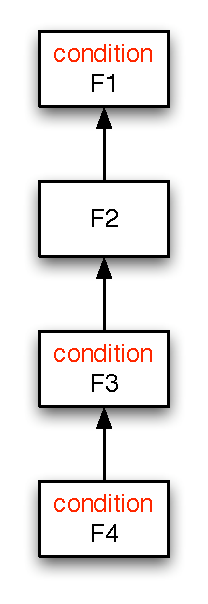
\includegraphics[scale=0.5]{depends_graph.eps}
\caption{Dependency graph model}
\label{fig:depends}
\end{minipage}
\hspace{0.5cm}
\begin{minipage}[b]{0.5\linewidth}
\centering
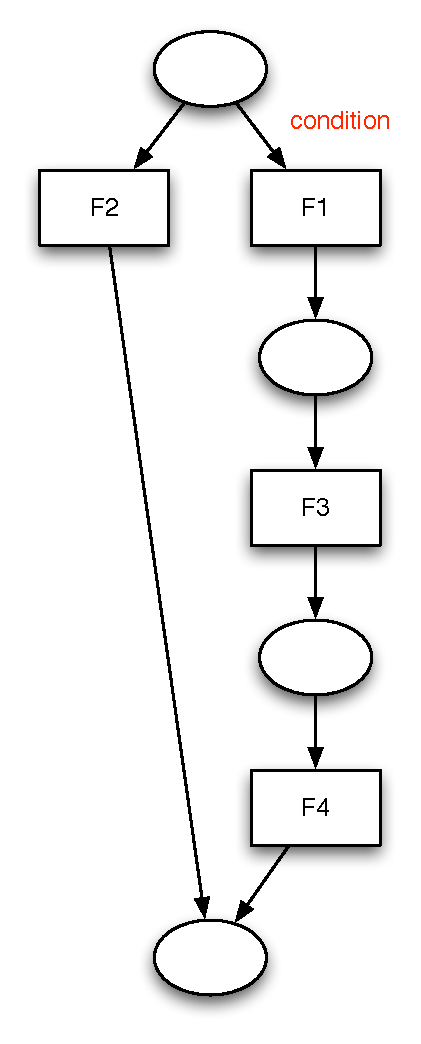
\includegraphics[scale=0.5]{state_graph.eps}
\caption{State graph model}
\label{fig:state}
\end{minipage}
\end{figure}

The model can now be recognised as a state machine but with the restriction
that once a state has been entered by an agent it cannot reenter the same
state. This provides synchronisation of agents in parallel during execution. Also
input to functions are sets of inputs (messages) which can be empty. This is
the level of detail required by FLAME to plan the communication synchronisation
in parallel.

Each function can then be defined by the parameters as shown in Table
\ref{tab:funcparameters}, where $M_{pre}$ is the pre-condition of the memory
and $M_{post}$ is the post-condition of the memory.

\begin{table}[hbp]
\centering
\begin{tabular}{|l|l|l||l||l|l|l|}
\hline
Current State&Input&$M_{pre}$&Function&$M_{post}$&Output&Next State\\
\hline
\end{tabular}
\caption{Function parameters} \label{tab:funcparameters}
\end{table}

In XMML this is currently written as below where $M_{pre}$ is defined as
\textit{condition} and $M_{post}$ is written as source code within a function
with the same name as the function name.

\begin{mylisting}
\begin{verbatim}
<function>
 <name>Function_name</name>
 <description>A description of the function</description>
 <currentState>current_state</currentState>
 <nextState>next_state</nextState>
 <condition>condition</condition>
 <inputs>inputs</inputs>
 <outputs>outputs</outputs>
</function>
\end{verbatim}
\end{mylisting}


%\section{Goods and Labour Market Implementation}

\section{State dependency graph}
\section{state transition table}
\section{Messages involved}
%\section{Credit Market Implementation}

This model was adapted from the proposed model of the credit market
by the Ancona Unit \cite{?}. Here we present a description of how
the model was implemented.

\subsection{Description}
The credit market involves the interaction of the credit function
with the financial management functions of the Firm and Bank agent.
The state dependency diagram \ref{fig:statecredit} shows the flow of
activity in the model.

% \subsection{Agents}
% The agents involved in the implementation are listed below:
% \begin{itemize}
% \item Bank Agent - reads loans requests and approves loans.
% \item Firm Agent - requests for loans if needed.
% \item Dummy Agent - to handle message of orders and household
% functions.
% \end{itemize}
%
% \subsection{State dependency diagram}
%
% \begin{figure}[!htb]
% \begin{center}
%  \includegraphics*[scale=2.0]{stategraph.ps}
% \caption{State Dependency Diagram.} \label{fig:statecredit}
% \end{center}
% \end{figure}
%
% The state dependency diagram \ref{fig:statecredit} shows the flow of
% activity in the model. The details of the functions of the agents
% can be found in the report presented by the Ancona Unit \cite{?}.
%
% The xmml file for the credit market can be found in the Chapter
% \ref{appendix}.
%
% \section{Results}
% Graphs


 \begin{figure}[!htb]
 \begin{center}
  \includegraphics*[scale=2.0]{stategraph.ps}
 \caption{State Dependency Diagram.} \label{fig:statecredit}
 \end{center}
 \end{figure}


\subsubsection{Firm Agent in the Credit Market}


\begin{landscape}
\begin{table}[!htb]\caption{Functions being performed by the Firm involved in Credit Market.}
\begin{center}
\begin{tabular}{|c|c|c|l|c|c|l|}
\hline
Function Name & State From & State to & Condition on Function & Inputs & Outputs & Description \\
\hline
{\parbox[l]{3cm}{Firm \_ask \_loan}}&
{\parbox[l]{3cm}{Start \_Firm \_Credit \_Role}}&
{\parbox[l]{3cm}{Firm \_Credit \_02}}&
{\parbox[l]{3cm}{a.external \_financial \_needs GT 0.0}}
&
&loan \_request &
\\
\hline

{\parbox[l]{3cm}{Firm \_get \_loan}}& {\parbox[l]{3cm}{Firm \_Credit
\_02}}& {\parbox[l]{3cm}{Firm \_End \_Credit \_Role}}&
&{\parbox[l]{3cm}{loan \_conditions ( a.id EQ m.firm\_id}} &
{\parbox[l]{3cm}{loan \_acceptance}}&\\
\hline


\end{tabular}\end{center}\label{tab:creditbankfn}
\end{table}
\end{landscape}

\subsubsection{Bank Agent in the Credit Market}



\begin{landscape}
\begin{table}[!htb]\caption{Functions being performed by the Bank involved in Credit Market.}
\begin{center}
\begin{tabular}{|c|c|c|l|c|c|l|}
\hline
Function Name & State From & State to & Condition on Function & Inputs & Outputs & Description \\
\hline

{\parbox[l]{3cm}{Bank \_decide \_credit \_conditions}} &
{\parbox[l]{3cm}{Bank \_start \_credit \_market \_role}} & Bank\_02
& & {\parbox[l]{3cm}{loan\_request (a.id EQ m.bank\_id)}} &
{\parbox[l]{3cm}{loan \_conditions}} &\\

\hline

{\parbox[l]{3cm}{Bank \_give \_loan}} & Bank\_02 & Bank\_03 & &
{\parbox[l]{3cm}{loan \_acceptance (a.id EQ m.bank \_id)}} &  &\\

\hline

{\parbox[l]{3cm}{Bank \_receive \_installment}} & Bank\_03 &
Bank\_04 & &
{\parbox[l]{3cm}{installment (a.id EQ m.bank\_id)}} & & \\

&&&&
{\parbox[l]{3cm}{bankruptcy (a.id EQ m.bank\_id)}} &  &\\

\hline


{\parbox[l]{3cm}{Bank \_account \_update \_deposits}} & Bank\_04 &
Bank\_05 & & {\parbox[l]{3cm}{bank\_account \_update (a.id EQ
m.bank\_id)}} &
{\parbox[l]{3cm}{central \_bank \_account \_update}} &\\

\hline


{\parbox[l]{3cm}{Bank \_accounting}} & Bank\_05 &
{\parbox[l]{3cm}{end \_Bank \_cycle}} &
{\parbox[l]{4cm}{monthly (a.day \_of \_month \_to \_act)}}&  &  &\\

\hline


{\parbox[l]{3cm}{Bank\_idle}} & Bank\_05 & {\parbox[l]{3cm}{end
\_Bank \_cycle}} &
{\parbox[l]{4cm}{not (monthly (a.day \_of \_month \_to \_act))}}&  &  &\\
\hline


\end{tabular}\end{center}\label{tab:creditbankfn}
\end{table}
\end{landscape}

\subsection{Messages being Used}



\begin{table}[!htb]\caption{Messages involved in the credit market implementation.}
\begin{center}
\begin{tabular}{|c|l|l|}
\hline
Name & Variables being sent & Description \\
\hline loan\_request & {\parbox[l]{5cm}{firm\_id, bank\_id, equity,
total\_debt, external\_financial\_needs}}& {\parbox[l]{5cm}{Message
added by firm to demand credit with bank\_id,
with financial info of applying firm.}} \\
\hline loan\_conditions & {\parbox[l]{5cm}{firm\_id, bank\_id,
proposed\_interest\_rate, amount\_offered\_credit, value\_at\_risk}}
& {\parbox[l]{5cm}{Message added by bank to offer credit, contains
the interest rate, the amount of
offered credit, and the value\_at\_risk.}}  \\

\hline loan\_acceptance & {\parbox[l]{5cm}{bank\_id,
credit\_amount\_taken, loan\_total\_var}} & {\parbox[l]{5cm}{Message
added by firm to accept a loan with bank\_id, for the amount credit
taken and VAR. The bank
does not need to know the firm\_id.}}   \\
\hline

installment & {\parbox[l]{5cm}{bank\_id, installment\_amount,
interest\_amount, var\_per\_installment}} & {\parbox[l]{5cm}{Message
added by firm pays
installment and interest to the bank.}}    \\

\hline bankruptcy & {\parbox[l]{5cm}{bank\_id, bad\_debt,
credit\_refunded, residual\_var}} &{\parbox[l]{5cm}{Message added by
firm to bank
to signal bankruptcy.}}  \\
\hline BCE\_return &
{\parbox[l]{5cm}{bce\_debt, id}} & {\parbox[l]{5cm}{}}  \\
\hline

\end{tabular}\end{center}\label{tab:creditmarketmsg}
\end{table}

%\subsection{Unit testing of the message board API}
As mentioned above the message boards (are accessed by the FLAME framework via a Application Program Interface - the Message Board Library (the libmboard API). This provides the FLAME developer with a uniform interface to the functionality of the libmboard.
\subsection{Testing serial and parallel implementations}
It is important to ensure that application generated by the FLAME framework execute \textsl{correctly} in both their serial and parallel modes. Because of the stocastic nature of the agent-based approach to modelling it is unrealistic to expect complex simulations to following exactly the solution path although general trends should be similar. However for some simple applications we can expect to serial and parallel implementations to produce exactly the results throughout the simulation. Such example applications can be used to verify the correctness of both the serial and parallel implementations.

The \textsl{Circles Model} is one such application. The \textsl{Circles} agent is very simple. It has a position in two-dimensional space and a radius of influence. Each agent will react to its neighbours within its interaction radius repulsively. So given a sufficient simulation time the initial distribution of agents will tend to a field of uniformly spaced agents. Each agent has $x$, $y$, $fx$, $fy$ and $radius$ in its memory and has three states: outputdata, inputdata and move. The agents communicate via a single message board, $location$, which holds the agent $id$ and position. Given the simplicity of the agent it is possible to determine the final result of a number of ideal models.

A set of simple test models and problems have been developed based on the \textsl{Circles} agent. Each test has a \textsl{model.xmml} files and a set of initial data (\textsl{0.xml}).
\begin{description}
	\item [Test 1]: Model: single \textsl{Circles} agent type; Initial population of no agents. Expected result:
	\item [Test 2]: Model: single \textsl{Circles} agent type; Initial population of one agent at (0,0).
	\item [Test 3]: Model: Two \textsl{Circles} agent type; Initial population of agents at (-1,0) and (+,0).
	\item [Test 4]: Model: Four \textsl{Circles} agent type; Initial population of one agent at ($\pm$1,$\pm$1).
	\item [Test 5]: Model: Four \textsl{Circles} agent type; Initial population of one agent at (0,$\pm$1) and ($\pm$1,0).
	\item [Test 6]: Model: Four \textsl{Circles} agent type; Initial population of one agent at random positions.
	\end{description}
In each of these models the expected results can be specified and therefore they provide a very simple check of the implementation.

The \textsl{Circles} agent also provides a good mechanism to check the parallel implementation against the serial. Such is the nature of the model the positions on the agents at each iteration of the simulation is independent on the order of calculation. As the order of calculation can not be easily prescript in the parallel simulation we can use this characteristic to test the validity of the parallel implementation against the serial. We would expect to get the identical positions for each agent at very iteration of the simulation.


%In this report we have described the parallel implementation of the FLAME framework and its assessment together with some benchmarking results using the EURACE Model. We have also demonstrated FLAMEs use in a number of EURACE related simulations in addition to complete EURACE model on populations ranging from a few hundereds of agents, through tens of thousands to, in one case, a million agents.  In some of these simulations the parallel implementation of FLAME has shown reasonable scalability and parallel efficiency but in other the results have been disappointing.

An important goal of the project has been to perform, in parallel, a large simulation using the EURACE Model. The project has achieve this to a degree: the model has been defined, important parameters have been values, a method of generating agent populations implemented and a parallel implementation of the EURACE model can be generated by FLAME. Using these steps serial and parallel simulations of the EURACE Model have been perform. In this process a detail assessment of the FLAME generated code, the serial and parallel implementations and the EURACE Model have been performed. Message counts, function times and sychronisation times are a few of the measures that have been used together with a detail static analysis of the model to identify the performance defficiencies in both the FLAME framework and the EURACE model.

All this analysis has lead to improvements in FLAME and the EURACE Model which in general have improved its computational performance. However the presence of substanial serial components in any model has resulted in very poor parallel scalability. It is well known that parallel speedup is limited by the serial faction of a code - this is Amdah's Law. The analyses performed on the EURACE Model have shown that the singleton agents - in particularly the Clearing House - have a significant impact of the parallel performance of the model.
These types of potential problem were understood - fine grained tasks - at the start of the project and the modeller took steps to avoid them. The Clearing House was thought necessary to the architecture of the EURACE Model and although different strategies were tested to reduce its effect there was little that could be achieved. The Clearing House and any other serial bottleneck will compromise the parallel performance of the application.

Although at the end of EURACE we have not achieved the \textsl{optimum} solution to these problems we have at least advanced the current state of the art in the parallel implementation of agent-based simulations in the context of the FLAME Framework.

%\bibliographystyle{alpha}
%\bibliographystyle{plain}
%\bibliography{EURACE_refs}
% End of document
\end{document}
